\section{Análise Exploratória}

A Análise Exploratória de Dados (AED) é uma etapa do fluxo de aprendizado de máquina que permite realizar uma exploração dos dados baseada em técnicas da Estatística Descritiva. Para essa etapa da pesquisa foi utilizado o notebook \textbf{analise-exploratoria.ipynb}. Por se tratar de uma atividade interativa, a utilização de um Jupyter Notebook se mostrou mais eficiente do que a utilização direta de um script Python.

\subsection{Valores Ausentes}

A primeira investigação realizada foi a busca de valores valores ausentes. Foram encontrados 1.900 segmentos com valores ausentes para o atributo txt\textunderscore seg. Nos demais atributos não havia valores ausentes. A tabela \ref{tab:valores-ausentes} apresenta a quantidade de segmentos com valores ausentes por tipo de segmento.

\begin{table}[h!] 
\caption{Valores ausentes por tipo de segmento}
\label{tab:valores-ausentes}
	\begin{center} 
		\begin{tabular}{|l|r|} 
			\hline TIPO DE SEGMENTO & VALORES AUSENTES \\
			\hline
			\hline Anexo & 1.778 \\
			\hline Não Identificado & 95 \\			
			\hline Fecho & 21 \\
			\hline Ementa & 2 \\			
			\hline Artigo & 2 \\
			\hline Título & 1 \\
			\hline Alínea & 1 \\			
			\hline
		\end{tabular}
	\end{center}
	\fdp
\end{table} 

Os segmentos do tipo Anexo representam 93,57\% dos segmentos com valores ausentes. Como esse tipo de segmento representa arquivos binários associados aos atos, todos os segmentos desse tipo podem ser descartados. Além dos 1.778 apresentados na tabela \ref{tab:valores-ausentes}, existem outros 5.771 segmentos do tipo anexo com texto desprezível (ponto, vírgula, nome de arquivo, etc) totalizando 7.549 segmentos selecionados para exclusão durante a etapa de limpeza de dados. Os demais segmentos com valores ausentes representam 0.06\% do total (122/198.939) e foram também selecionados para exclusão.

\subsection{Distribuições de Atos e Segmentos}

Um aspecto que chamou a atenção na exploração dos dados foi a predominância de Atos Declaratórios Executivos (ADE), representando 71,79\% (14.948 dos 20.821 atos analisados), seguido pelas Soluções de Consulta (SC) com 14,98\% e Portarias (Port.) com 10,60\%. Os demais tipos de ato representam juntos 2.63\% do total. A figura \ref{fig:atos-por-tipo-ato} evidencia essa distribuição.

\begin{figure}[h]
	\caption{Quantidade de atos por tipo de ato}
	\center
	\label{fig:atos-por-tipo-ato}
	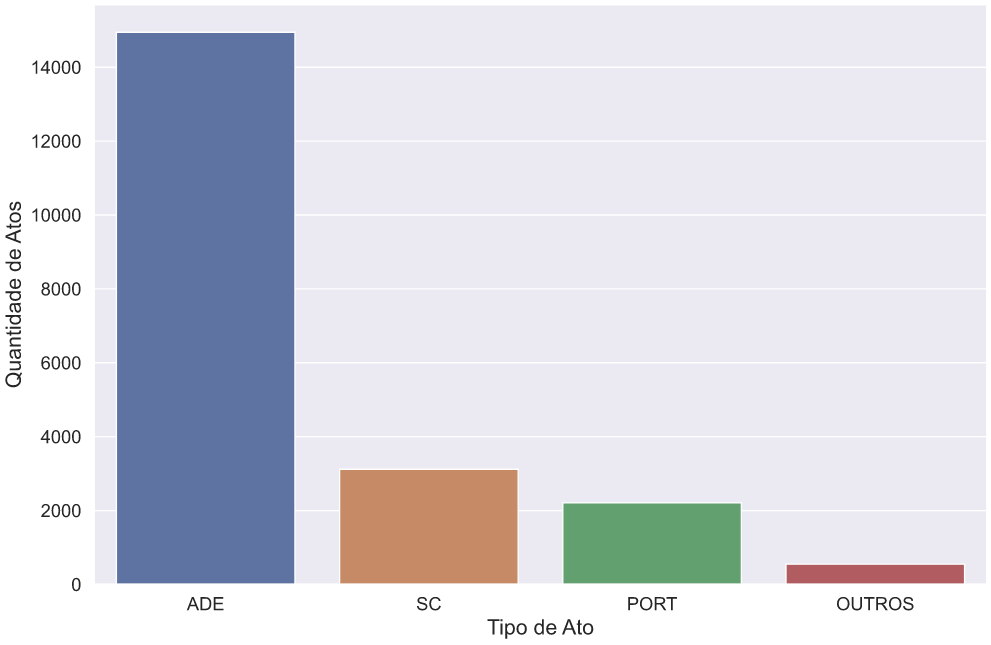
\includegraphics[scale=1.7]{exploratoria/atos-por-tipo-ato.png}
	\fdp
\end{figure}

Outro aspecto importante analisado durante a exploração de dados foi distribuição dos segmentos por tipo de ato.

 \begin{figure}[h]
	\caption{Distribuição dos segmentos por tipo de ato}
	\center
	\label{fig:segmentos-por-tipo-ato}
	\includegraphics[scale=1.7]{exploratoria/segmentos-por-tipo-ato.png}
	\fdp
\end{figure}

